\documentclass{statsmsc}

\title{Statistics Research Project Title}
\author{FIRSTNAME LASTNAME}
\CID{01234567}
\supervisor{SUPERVISORNAME and COSUPERVISORNAME}
\date{1 May 2025}
%For today's date, use:
%\date{\today}
\logoimg{}

% THIS IS WHERE NEW COMMANDS CAN BE DEFINED

% commands below only used in the proof; otherwise can be deleted
\newcommand{\consta}{a}
\newcommand{\X}{X}
\newcommand{\EE}[1]{ \mathrm{E} [ #1 ] }
\newcommand{\inparenth}[1]{\left( #1 \right)}

\usepackage{xcolor}
\usepackage{hyperref}
\hypersetup{
    colorlinks,
    linkcolor={blue!50!black},
    citecolor={blue!50!black},
    urlcolor={blue!50!black}
}


\begin{document}

% Generates the Title Page
\maketitle

% Generates plagiarism declaration
\declarationname{STUDENT'S NAME}
\declarationdate{DATE}
\declaration 

\begin{acknowledgements}
    In the acknowledgments, you should account for anyone who supported you during your research. This could include family, your research peer group, other students, research group members, your supervisor, data providers, external partners, any computing service used, any financial support. 
    
    If your research peer group, other students, research group members, or your supervisors made substantive contributions towards your report -- e.g. they identified suitable methods, provided code or contributed a sub-analysis -- you must acknowledge their precise contribution here.
\end{acknowledgements}

%=================================================================
% VERY IMPORTANT
% This command switches from Roman to Arabic numbering for main part of report. Do not modify.
\mainmatter
%=================================================================


\begin{abstract}
    Abstracts should be no longer than 300 words, and similar in style to a general science or statistics research paper.
\end{abstract}

%===============================================================
%
% Students please remove the General tips when submitting your report
%
%===============================================================
\paragraph{General tips.} Your research report will be judged on the quality of the work it describes according to the Marking Criteria shared with you. 
When writing your research report you may assume that the reader is familiar with the four core modules of the MSc in statistics. Any additional other material should be explained to the reader, providing suitable references. See Section~\ref{sec:referencing} for more details. For example, you should avoid writing up in detail statistical methods discussed in one of the four core modules, but instead you should briefly present such methods and add appropriate references. More advanced methods or methods discussed in one of the elective modules should be described in more detail and referenced appropriately. 

Your report must be presented within this template and be at most 35 pages in length, as counted by the Arabic page numerals (1,2,3…). This limit includes all figures and tables presented in the main text, excluding the Endmatter and References sections. This is approximately equivalent to a limit of 15,000 words. Shorter submissions may be graded highly, while excess length disproportionate to the content may be penalised.


Before submitting the research project, make sure you read the report in its entirety. There should be no half-finished sentences. All mathematical symbols should be defined. Use a spell-checker.

You will have to submit your report electronically in PDF format through the virtual learning environment (Blackboard). Please name this file in the following format: “CID-Surname-Firstname-Report.pdf”. Your report will be checked for plagiarism via online plagiarism detection services (e.g. Turnitin). 

Note the report submission deadline is a very hard deadline since the assessment process has then to be completed on a very short timescale.

\section{Introduction}
\paragraph{Tips for the Introduction.} This is where you describe the topic and the research objectives of your project. 

You should attempt to set your work in the context of other work previously done in the field. Convey the background of your research referencing earlier work as appropriate. Define core terms. Include background and context, and focus as appropriate on the wider statistical context. Aim to demonstrate that you can confidently describe your project within a broader context of statistical research, as well as scientific research, that goes well beyond the more narrow topic of your project.


The introduction needs to demonstrate that you are aware of what you are doing, and how it relates to other work that should be properly referenced. 

Clearly point out your main contributions at the end of the introduction, and provide an overview how the rest of your report is structured and links together. 

Aim for approximately 1.5-3 pages, similar in style to a general science or statistics research paper.\footnote{Tip: If you choose to use footnotes, do so sparingly.}.





\section{Methods}\label{sec:methods}


\paragraph{Tips for the Methods section.} In general, you may structure the main body of your report in a form that suits your project best. We recommend to start with a substantial Methods section that includes, as in a research paper, a description of the following:
\begin{itemize}
    \item Key definitions and setting using mathematical notation. Any terminology related to the topic/data needs to be clearly presented and explained to the reader.
    \item Any data used in the project should be clearly explained in sufficient detail in the Methods section so that readers can follow the rest of your report without the need to consult an other report or any of your references.
    \item If in the project you have generated simulated data, a clear presentation of the generative procedure needs to be included. 
    \item Background statistical work using mathematical notation.
    \item All maths should be presented in inline or display formulas with appropriate referencing. For example, use $\exp(x)$ not exp(x) and $\sin(\theta)$ not $sin(\theta)$ or sin($\theta$). Display formulas should be numbered using the equation environment if they are referenced in the main text. Display equation blocks should be numbered using the subequations environment:
\begin{subequations}\label{eq:Y}
    \begin{align}
        Y & = 1 + Z \label{eq:Y1} \\ 
        Z & \sim \mathcal{N}(0,1) \label{eq:Y2},
    \end{align}
\end{subequations}
    so that you can reference~\eqref{eq:Y}, ~\eqref{eq:Y1}, and ~\eqref{eq:Y2}.
    \item If your main findings are of an applied nature, you may prefer to describe any new/original statistical procedures or models here. Include the key derivations and proofs if there are any, and any supplementary derivations in the appendix. Clearly highlight your contribution relative to existing work. 
    \item If your main findings are of a theoretical nature, you may prefer to describe any new/original statistical procedures or models in the Results section.
    \item Structure your Methods section using LaTeX   subsections and reference them using labels.
    \item Aim for approximately 8-15 pages, similar in style to a general science or statistics research paper.
\end{itemize}


\subsection{My Methods subsection}\label{subsec:my_subsec}

This text is in Subsection~\ref{subsec:my_subsec}, which is a part of Section~\ref{sec:methods}.

\subsubsection{My subsubsection}
If needed, subsections can also have subsubsections within them. Keep subsections and subsubsections numbered, which will help us to reference them.


\paragraph{Paragraphs.} In the rare event that you need a more deeply nested structure within a subsubsection, the \texttt{\textbackslash paragraph\{\}} command can be useful. 

\section{Results}

\paragraph{Tips for the Results section.} 

\begin{itemize}
    \item If your main findings are of a theoretical nature, you may prefer to describe any new/original statistical procedures or models in the Results section.
    \item Describe your findings concisely and precisely using scientific language. 
    \item Include sound interpretations and explanations wherever possible to demonstrate your original and clear statistical thought process. 
    \item Use figures and tables to support your main arguments, which should include a caption describing, e.g., what is shown on the $x-$ and $y$-axis or in the rows and columns. Summarise the main finding or headline numbers in the main text, including references to Figures and Tables as needed. Do not report all numbers shown in a figure or table.
    \item Include references to previous work as needed. 
    \item Structure your Results section into numbered Subsections and Subsubsections as needed, and feel free to reference these throughout.
    \item Aim for approximately 5-15 pages, similar in style to a general science or statistics research paper.
\end{itemize}

\section{Discussion}

\paragraph{Tips for the Discussion section.} 

\begin{itemize}
    \item Begin your Discussion with a summary and the main findings of your research in 2-5 sentences.
    \item Describe the implications of your main findings in the context of existing work concisely and precisely using scientific language. 
    \item Describe the limitations in your statistical methods and your main findings. Be honest about the limitations in your approach, and substantiate what could have been done differently as needed. Explain if your main findings are robust or sensitive to these limitations.
    \item Avoid Subsections and Subsubsections in the Discussion.
    \item In the last paragraph, conclude your report with a pitch using plain language that summarises the key implications of your research in the context of previous work. Write this last paragraph for the Imperial Press Office or journalists as audience.
    \item Aim for approximately 1-3 pages, similar in style to a general science or statistics research paper.
\end{itemize}

\section{Endmatter} \label{sec:endmatter}

\paragraph{Tips for the Endmatter section.} 

\begin{itemize}
    \item Include a data availability statement. Examiners must be able to reproduce your analyses on all the data investigated as would be the case during peer review of a research paper.
    \item Include a reproducibility statement, including the URL under which your code can be found. Examiners must be able to see your code, and they must be able to run your code.
\end{itemize}

%=========================================================
%
%
%
% Students should not edit below here 
%
%
%
%=========================================================

%=========================================================
%% Create bibliography
%
% - Add your references by modifying the file `refs.bib`
%
%=========================================================

\clearpage

%%References part of the main text
% References: modify the file refs.bib
\bibliographystyle{apalike}
\bibliography{refs}

\clearpage

%=========================================================
%% Create supplementary material 
%
%
% - Providing supplementary materials to your report is voluntary and will not normally be read by your examiners.
% - If you wish to include supplementary materials, add these by modifying the file 
%   `supplementary.tex`
% - otherwise deactive the include command below
%
%
%=========================================================

%% reset page counter and start appendix pages numbering
\pagenumbering{arabic}
\renewcommand*{\thepage}{Supplementary Material Page \arabic{page}}
\renewcommand{\thesection}{\Alph{section}}
%% Supplementary Material goes here
\appendix
\pagebreak
\section*{Supplementary Materials}
\begin{figure}[H]
\centering
\begin{subfigure}[t]{0.64\textwidth}
  \centering
  \includegraphics[height=4.5cm, width=\textwidth]{images/.pdf}  % 图1路径
  \caption{{\small ECDFs}}
  \label{fig:ecdf-event_a30}
\end{subfigure}
\begin{subfigure}[t]{0.351\textwidth}
\centering
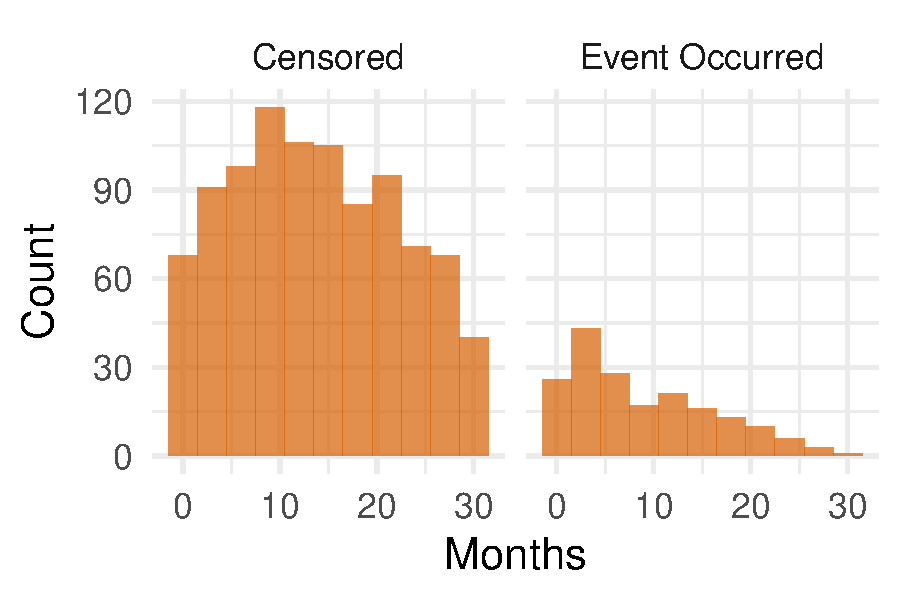
\includegraphics[height=4.5cm,width=\linewidth]{images/fake_duration_hist_a30.pdf}   % 图3路径
\caption{{\small Fake-data histogram}}
\label{fig:fake-hist_a30}
\end{subfigure}
\caption{{\small Posterior predictive checking ($A=30$).}}
\label{fig:ppc-A30}
\end{figure}

%=========================================================


\end{document}
